\documentclass{article}			% Try book, report etc.

\usepackage[utf8]{inputenc}		% Character encoding
\usepackage[T1]{fontenc}		% Font encoding
\usepackage[english]{babel}		% Language setting
\usepackage{enumerate}			% Custom enumeration lists
\usepackage{natbib}				% Harvard-style bibliography with several options
\usepackage{float}				% Custom table and figure alignment
\usepackage{multirow}			% Multiple rows in a table
\usepackage{hyperref}			% References
\usepackage{makecell}			% Custom table lines
\usepackage{subfig}				% Subfigures
\usepackage{tikz}				% TikZ drawings
\usepackage{pgfplots}			% PGFPlots plots
\pgfplotsset{					% PGFPlots options
	standard/.style={			% Declaring Cartesian plane style
		% Axis alignment
        axis x line=middle,
        axis y line=middle,
        % Axis labels alignment
        every axis x label/.style={at={(current axis.right of origin)},anchor=north west},
        every axis y label/.style={at={(current axis.above origin)},anchor=north east},
        % Legend alignment
        every axis legend/.append style={legend pos=outer north east}
    },
    compat=1.8					% Version declaration for compatibility
}
\hypersetup{					% Setup for this package
    colorlinks,
    citecolor=black,
    filecolor=black,
    linkcolor=black,
    urlcolor=blue
}

\usepackage{amsmath}		% AMS math package, with bugfixes in mathtools
\usepackage{amssymb}			% Math symbols
\usepackage{amsthm}				% Custom theorem environments
\usepackage{units}				% Numerical fractions

% Custom theorems
%\newtheorem{codename}[counter]{Display name}
\newtheorem{theorem}{Theorem}[]
\newtheorem{acknowledgement}[theorem]{Acknowledgment}
\newtheorem{algorithm}[theorem]{Algorithm}
\newtheorem{axiom}[theorem]{Axiom}
\newtheorem{case}[theorem]{Case}
\newtheorem{claim}[theorem]{Claim}
\newtheorem{conclusion}[theorem]{Conclusion}
\newtheorem{condition}[theorem]{Condition}
\newtheorem{conjecture}[theorem]{Conjecture}
\newtheorem{corollary}[theorem]{Corollary}
\newtheorem{criterion}[theorem]{Criterion}
\newtheorem{definition}[theorem]{Definition}
\newtheorem{exercise}[theorem]{Exercise}
\newtheorem{lemma}[theorem]{Lemma}
\newtheorem{notation}[theorem]{Notation}
\theoremstyle{definition}
\newtheorem{problem}[theorem]{Problem}
\newtheorem{assumption}[theorem]{Assumption}
\newtheorem{proposition}[theorem]{Proposition}
\theoremstyle{remark}
\newtheorem{example}[theorem]{Example}
\newtheorem{remark}[theorem]{Remark}
\newtheorem{solution}[theorem]{Solution}
\newtheorem{summary}[theorem]{Summary}

%\renewcommand{\qedsymbol}{$\blacksquare$}

\title{Graphics in \LaTeX}			% This is how the symbol for LaTeX and TeX are typeset
\author{Attila Gyetvai}

%%%%%%%%%%%%%%%%%%%%%%%%%%%%%%%%%

\begin{document}

\maketitle						% If date is not specified, current date is included; for no 										  date, write \date{}

\section{Including premade graphics}

One can include pre-made graphics: \includegraphics[scale=0.2]{ceu-logo.jpg}

The environment for any graphics is figure:

\begin{figure}[H]
\centering
\includegraphics[scale=0.2]{ceu-logo.jpg}
\caption{The logo of CEU.}
\end{figure}

You can put multiple graphics in one figure environment:

\begin{figure}[H]
\centering
\subfloat[CEU]{\includegraphics[scale=0.2]{ceu-logo.jpg}}
\subfloat{\includegraphics[scale=1]{economics.png}} \\
\subfloat[Math]{\includegraphics[scale=0.05]{math.jpg}}
\caption{Multiple images in one figure.}
\end{figure}

\section{Introduction to Ti\emph{k}Z}

\begin{figure}[H]
\centering
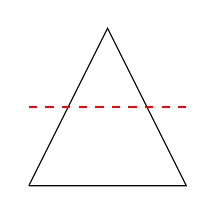
\begin{tikzpicture}[scale=1]
	\draw (0,0) -- (1,2) -- (2,0) -- (0,0);
	\draw[thick,red,dashed] (0,1) -- (2,1);
\end{tikzpicture}
\caption{My first Ti\emph{k}Z picture}
\end{figure}

\begin{figure}[H]
\centering
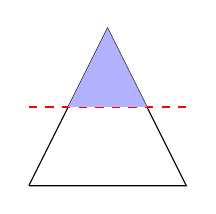
\begin{tikzpicture}[scale=1]
	\draw (0,0) coordinate (a) -- (1,2) coordinate (b) -- (2,0) coordinate (c) -- (a);
	\draw[thick,red,dashed] (0,1) coordinate (d) -- (2,1) coordinate (e);
	\fill[blue!30!white] (intersection of a--b and d--e) -- (b) -- (intersection of b--c and d--e);
\end{tikzpicture}
\caption{My second Ti\emph{k}Z picture}
\end{figure}

\begin{figure}[H]
\centering
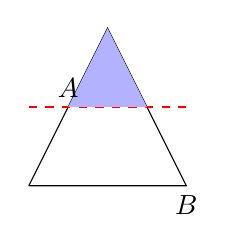
\begin{tikzpicture}[scale=1]
	\draw (0,0) coordinate (a) -- (1,2) coordinate (b) -- (2,0) coordinate (c) -- (a);
	\draw[thick,red,dashed] (0,1) coordinate (d) -- (2,1) coordinate (e);
	\fill[blue!30!white] (intersection of a--b and d--e) coordinate (f) -- (b) -- (intersection of b--c and d--e) coordinate (g);
	\node[left,above] at (f) {$A$};
	\node[right,below] at (c) {$B$};
\end{tikzpicture}
\caption{Labeling stuff in Ti\emph{k}Z}
\end{figure}

\section{Introduction to PGFPlots}

\begin{figure}[H]
\centering
\begin{tikzpicture}
\begin{axis}
	\addplot [domain=-1:1] {abs(x)};
	\addplot [domain=-1:1] {exp(x)};
\end{axis}
\end{tikzpicture}
\caption{My first PGFPlots plot}
\end{figure}

\begin{figure}[H]
\centering
\begin{tikzpicture}
\begin{semilogyaxis}
	\addplot [domain=0:1] {x};
	\addplot [domain=0:1] {exp(x)};
\end{semilogyaxis}
\end{tikzpicture}
\caption{Logarithmic axes in PGFPlots}
\end{figure}

\begin{figure}[H]
\centering
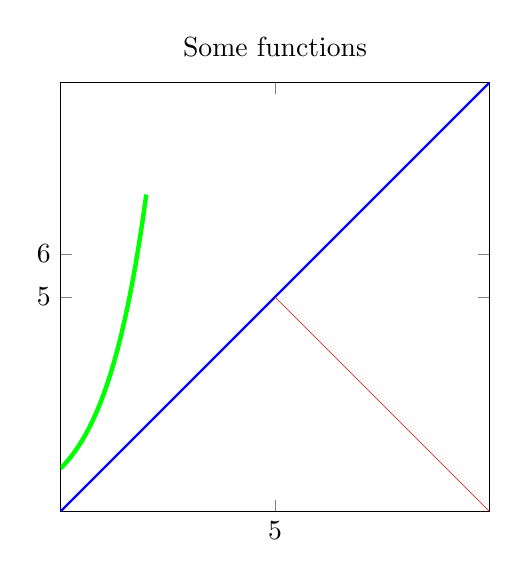
\begin{tikzpicture}
\begin{axis}[
    xmin=0, xmax=10,
    ymin=0, ymax=10,
    xtick={5}, ytick={5,6},
    height=20em, width=20em,
    title=Some functions
]
	\addplot [blue, thick, domain=0:10] {x};
	\addplot [red, very thin, domain=5:10] {10-x};
	\addplot [green, ultra thick, domain=0:2] {exp(x)};
\end{axis}
\end{tikzpicture}
\caption{Options for axes and plots in PGFPlots}
\end{figure}

\begin{figure}[H]
\centering
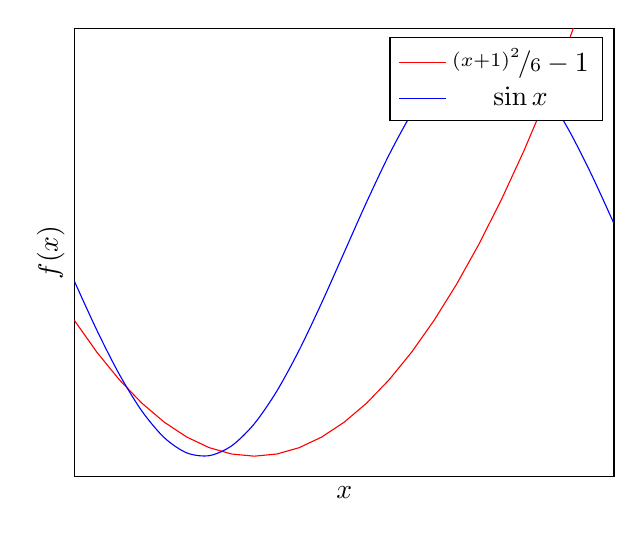
\begin{tikzpicture}
\begin{axis}[
%	standard,
	xmin=-3, xmax=3,
	ymin=-1.1, ymax=1.1,
	ticks=none,
	xlabel=$x$, ylabel=$f(x)$
]
	\addplot [red, domain=-3:3] {(x+1)^2/6 -1};
	\addplot [blue, smooth, domain=-3:3] {sin(deg(x))};
	\legend{$\nicefrac{(x+1)^2}{6} -1$,$\sin x$};
\end{axis}
\end{tikzpicture}
\caption{A classic Cartesian coordinate plane}
\end{figure}

\begin{figure}[H]
\centering
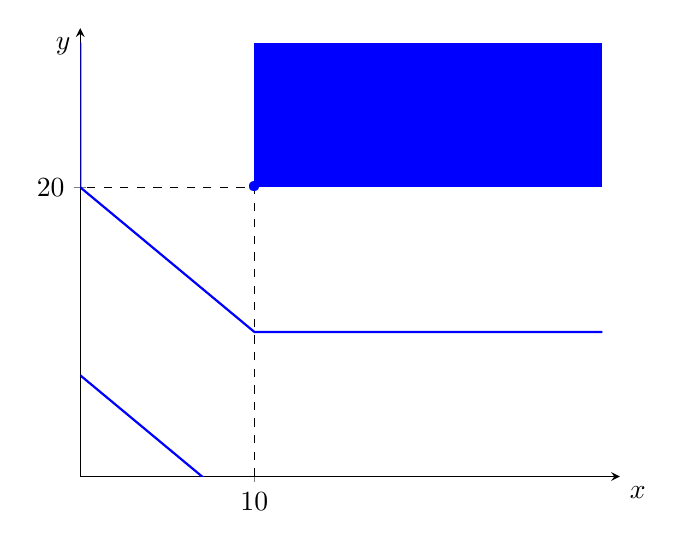
\begin{tikzpicture}
\begin{axis}[
    standard,
    xmin=0, xmax=31,
    ymin=0, ymax=31,
    xtick={10}, ytick={20},
    xlabel=$x$, ylabel=$y$
]
	\addplot [dashed] coordinates {(10,0) (10,20) (0,20)};
	\addplot [thick, blue, domain=0:10] {7-x};
	\addplot [thick, blue, domain=0:10] coordinates {(0,30) (0,20) (10,10) (30,10)};
	\fill [blue]  (axis cs:10,20) -- (axis cs:30,20) -- (axis cs:30,30) -- (axis cs:10,30);
	\node [blue] at (axis cs:10,20) {\textbullet};
\end{axis}
\end{tikzpicture}
\caption{A familiar figure.}
\end{figure}

\begin{figure}[H]
\centering
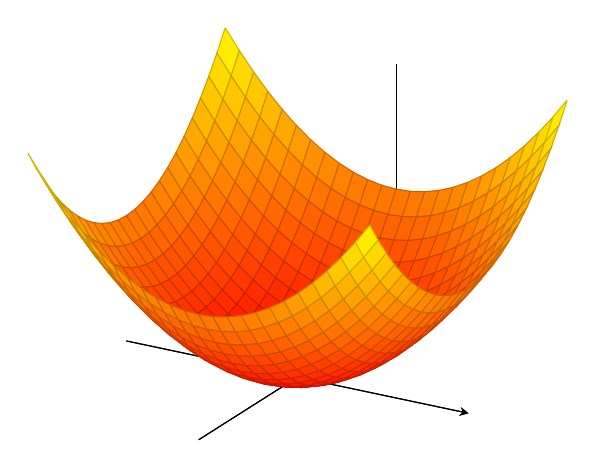
\begin{tikzpicture}
\begin{axis}[
	standard,
	xmin=-5, xmax=5,
	ymin=-5, ymax=5,
	zmin=0, zmax=50,
	ticks=none,
	colormap/redyellow,
	view={30}{30}
]
	\addplot3 [surf] {x^2 + y^2};
\end{axis}
\end{tikzpicture}
\caption{3D plot in PGFPlots}
\end{figure}

\end{document}